\documentclass{standalone}
\usepackage{tikz}
\usetikzlibrary{patterns, positioning}


\begin{document}
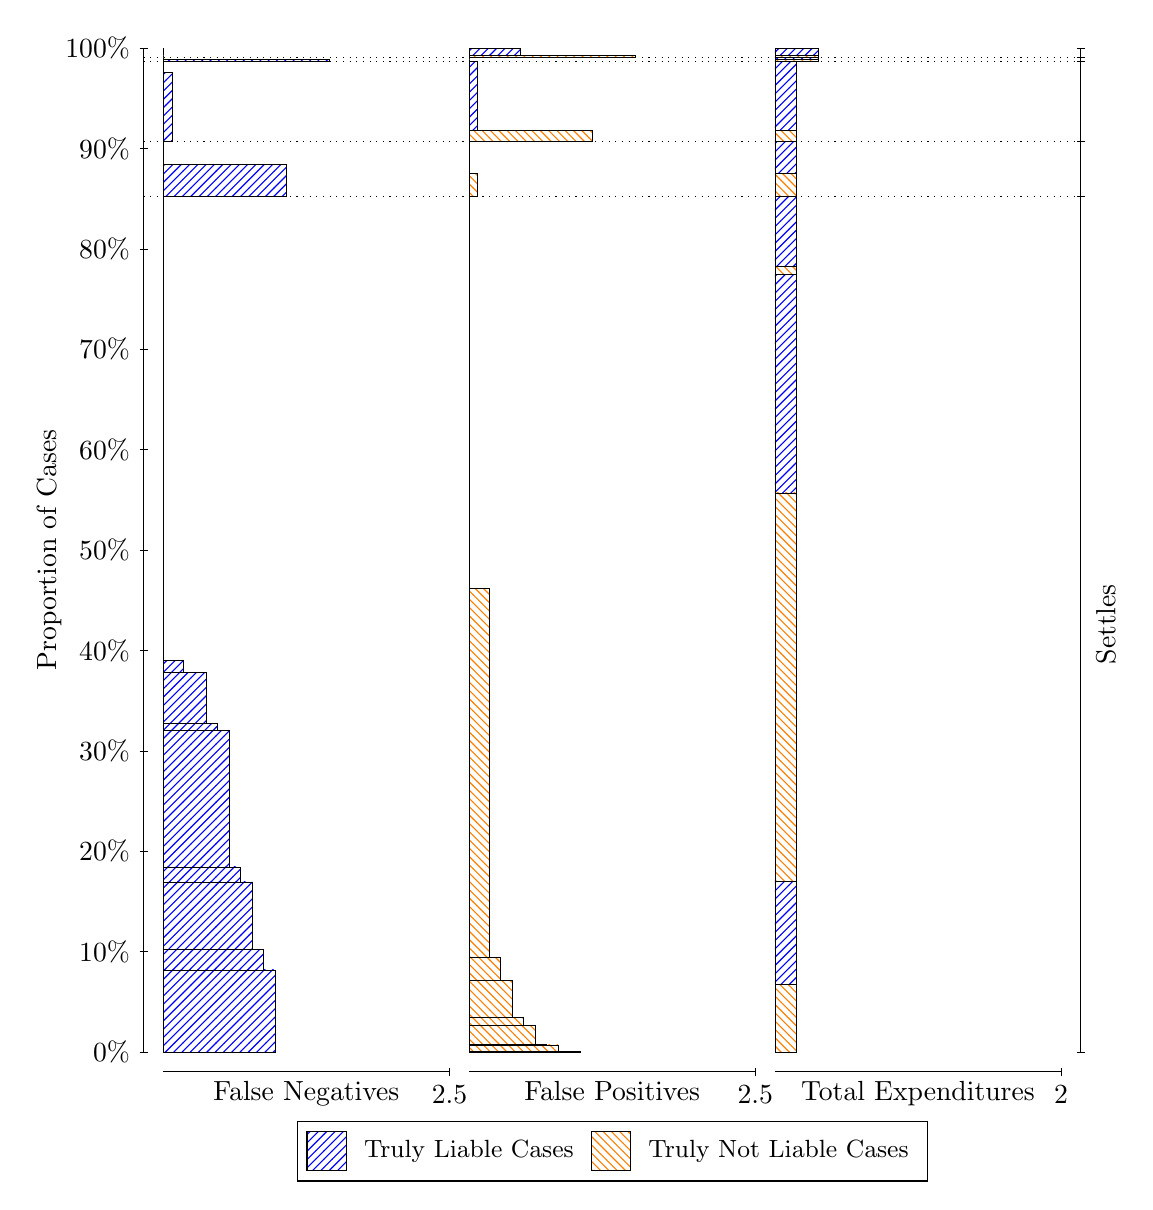
\begin{tikzpicture}
\draw[black, very thin] (1.5,1.75) -- (1.5,14.5);
\node[rotate=90, text=black, anchor=center] at (0.3, 8.125) {Proportion of Cases};
\draw[black, very thin] (1.45,1.75) -- (1.55,1.75);
\node[text=black, anchor=east] at (1.45, 1.75) {0\%};
\draw[black, very thin] (1.45,3.025) -- (1.55,3.025);
\node[text=black, anchor=east] at (1.45, 3.025) {10\%};
\draw[black, very thin] (1.45,4.3) -- (1.55,4.3);
\node[text=black, anchor=east] at (1.45, 4.3) {20\%};
\draw[black, very thin] (1.45,5.575) -- (1.55,5.575);
\node[text=black, anchor=east] at (1.45, 5.575) {30\%};
\draw[black, very thin] (1.45,6.85) -- (1.55,6.85);
\node[text=black, anchor=east] at (1.45, 6.85) {40\%};
\draw[black, very thin] (1.45,8.125) -- (1.55,8.125);
\node[text=black, anchor=east] at (1.45, 8.125) {50\%};
\draw[black, very thin] (1.45,9.4) -- (1.55,9.4);
\node[text=black, anchor=east] at (1.45, 9.4) {60\%};
\draw[black, very thin] (1.45,10.675) -- (1.55,10.675);
\node[text=black, anchor=east] at (1.45, 10.675) {70\%};
\draw[black, very thin] (1.45,11.95) -- (1.55,11.95);
\node[text=black, anchor=east] at (1.45, 11.95) {80\%};
\draw[black, very thin] (1.45,13.225) -- (1.55,13.225);
\node[text=black, anchor=east] at (1.45, 13.225) {90\%};
\draw[black, very thin] (1.45,14.5) -- (1.55,14.5);
\node[text=black, anchor=east] at (1.45, 14.5) {100\%};

\draw[black, very thin] (13.4,1.75) -- (13.4,14.5);
\draw[black, very thin] (13.35,1.75) -- (13.45,1.75);
\node[anchor=west] at (13.35, 1.75) {};
\draw[black, very thin] (13.35,12.615) -- (13.45,12.615);
\node[anchor=west] at (13.35, 12.615) {};
\draw[black, very thin] (13.35,13.315) -- (13.45,13.315);
\node[anchor=west] at (13.35, 13.315) {};
\draw[black, very thin] (13.35,14.332) -- (13.45,14.332);
\node[anchor=west] at (13.35, 14.332) {};
\draw[black, very thin] (13.35,14.381) -- (13.45,14.381);
\node[anchor=west] at (13.35, 14.381) {};
\draw[black, very thin] (13.35,14.5) -- (13.45,14.5);
\node[anchor=west] at (13.35, 14.5) {};

\draw[black, very thin, pattern color=blue, pattern=north east lines] (1.75,1.75) rectangle (3.167,2.7914);
\draw[black, very thin, pattern color=blue, pattern=north east lines] (1.75,2.7914) rectangle (3.0217,3.0488);
\draw[black, very thin, pattern color=blue, pattern=north east lines] (1.75,3.0488) rectangle (2.8763,3.9114);
\draw[black, very thin, pattern color=blue, pattern=north east lines] (1.75,3.9114) rectangle (2.731,4.0998);
\draw[black, very thin, pattern color=blue, pattern=north east lines] (1.75,4.0998) rectangle (2.5857,5.8365);
\draw[black, very thin, pattern color=blue, pattern=north east lines] (1.75,5.8365) rectangle (2.4403,5.9209);
\draw[black, very thin, pattern color=blue, pattern=north east lines] (1.75,5.9209) rectangle (2.295,6.5736);
\draw[black, very thin, pattern color=blue, pattern=north east lines] (1.75,6.5736) rectangle (2.0043,6.7247);
\draw[black, very thin, pattern color=orange, pattern=north west lines] (1.75,6.7247) rectangle (1.75,12.615);
\draw[black, very thin, pattern color=blue, pattern=north east lines] (1.75,12.615) rectangle (3.3123,13.018);
\draw[black, very thin, pattern color=orange, pattern=north west lines] (1.75,13.018) rectangle (1.75,13.315);
\draw[black, very thin, pattern color=blue, pattern=north east lines] (1.75,13.315) rectangle (1.859,14.193);
\draw[black, very thin, pattern color=orange, pattern=north west lines] (1.75,14.193) rectangle (1.75,14.332);
\draw[black, very thin, pattern color=blue, pattern=north east lines] (1.75,14.332) rectangle (3.8573,14.357);
\draw[black, very thin, pattern color=orange, pattern=north west lines] (1.75,14.357) rectangle (1.75,14.381);
\draw[black, very thin, pattern color=orange, pattern=north west lines] (1.75,14.381) rectangle (1.75,14.406);
\draw[black, very thin, pattern color=blue, pattern=north east lines] (1.75,14.406) rectangle (1.75,14.5);
\draw[black, very thin, pattern color=orange, pattern=north west lines] (5.6333,1.75) rectangle (7.0503,1.761);
\draw[black, very thin, pattern color=orange, pattern=north west lines] (5.6333,1.761) rectangle (6.7597,1.8387);
\draw[black, very thin, pattern color=orange, pattern=north west lines] (5.6333,1.8387) rectangle (6.6143,1.8479);
\draw[black, very thin, pattern color=orange, pattern=north west lines] (5.6333,1.8479) rectangle (6.469,2.0925);
\draw[black, very thin, pattern color=orange, pattern=north west lines] (5.6333,2.0925) rectangle (6.3237,2.1897);
\draw[black, very thin, pattern color=orange, pattern=north west lines] (5.6333,2.1897) rectangle (6.1783,2.6605);
\draw[black, very thin, pattern color=orange, pattern=north west lines] (5.6333,2.6605) rectangle (6.033,2.954);
\draw[black, very thin, pattern color=orange, pattern=north west lines] (5.6333,2.954) rectangle (5.8877,7.6401);
\draw[black, very thin, pattern color=blue, pattern=north east lines] (5.6333,7.6401) rectangle (5.6333,12.615);
\draw[black, very thin, pattern color=orange, pattern=north west lines] (5.6333,12.615) rectangle (5.7423,12.912);
\draw[black, very thin, pattern color=blue, pattern=north east lines] (5.6333,12.912) rectangle (5.6333,13.315);
\draw[black, very thin, pattern color=orange, pattern=north west lines] (5.6333,13.315) rectangle (7.1957,13.453);
\draw[black, very thin, pattern color=blue, pattern=north east lines] (5.6333,13.453) rectangle (5.7423,14.332);
\draw[black, very thin, pattern color=orange, pattern=north west lines] (5.6333,14.332) rectangle (5.6333,14.356);
\draw[black, very thin, pattern color=blue, pattern=north east lines] (5.6333,14.356) rectangle (5.6333,14.381);
\draw[black, very thin, pattern color=orange, pattern=north west lines] (5.6333,14.381) rectangle (7.7407,14.406);
\draw[black, very thin, pattern color=blue, pattern=north east lines] (5.6333,14.406) rectangle (6.2873,14.5);
\draw[black, very thin, pattern color=orange, pattern=north west lines] (9.5167,1.75) rectangle (9.7892,2.6114);
\draw[black, very thin, pattern color=blue, pattern=north east lines] (9.5167,2.6114) rectangle (9.7892,3.9198);
\draw[black, very thin, pattern color=orange, pattern=north west lines] (9.5167,3.9198) rectangle (9.7892,8.8506);
\draw[black, very thin, pattern color=blue, pattern=north east lines] (9.5167,8.8506) rectangle (9.7892,11.629);
\draw[black, very thin, pattern color=orange, pattern=north west lines] (9.5167,11.629) rectangle (9.7892,11.727);
\draw[black, very thin, pattern color=blue, pattern=north east lines] (9.5167,11.727) rectangle (9.7892,12.615);
\draw[black, very thin, pattern color=orange, pattern=north west lines] (9.5167,12.615) rectangle (9.7892,12.912);
\draw[black, very thin, pattern color=blue, pattern=north east lines] (9.5167,12.912) rectangle (9.7892,13.315);
\draw[black, very thin, pattern color=orange, pattern=north west lines] (9.5167,13.315) rectangle (9.7892,13.453);
\draw[black, very thin, pattern color=blue, pattern=north east lines] (9.5167,13.453) rectangle (9.7892,14.332);
\draw[black, very thin, pattern color=orange, pattern=north west lines] (9.5167,14.332) rectangle (10.062,14.356);
\draw[black, very thin, pattern color=blue, pattern=north east lines] (9.5167,14.356) rectangle (10.062,14.381);
\draw[black, very thin, pattern color=orange, pattern=north west lines] (9.5167,14.381) rectangle (10.062,14.406);
\draw[black, very thin, pattern color=blue, pattern=north east lines] (9.5167,14.406) rectangle (10.062,14.5);
\draw[black, dotted] (1.5,12.615) -- (13.4,12.615);
\draw[black, dotted] (1.5,13.315) -- (13.4,13.315);
\draw[black, dotted] (1.5,14.332) -- (13.4,14.332);
\draw[black, dotted] (1.5,14.381) -- (13.4,14.381);
\draw[black, very thin] (1.75,1.5) -- (5.3833,1.5);
\node[text=black, anchor=north] at (3.5667, 1.5) {False Negatives};
\draw[black, very thin] (5.3833,1.45) -- (5.3833,1.55);
\node[text=black, anchor=north] at (5.3833, 1.45) {2.5};

\draw[black, very thin] (5.6333,1.5) -- (9.2667,1.5);
\node[text=black, anchor=north] at (7.45, 1.5) {False Positives};
\draw[black, very thin] (9.2667,1.45) -- (9.2667,1.55);
\node[text=black, anchor=north] at (9.2667, 1.45) {2.5};

\draw[black, very thin] (9.5167,1.5) -- (13.15,1.5);
\node[text=black, anchor=north] at (11.333, 1.5) {Total Expenditures};
\draw[black, very thin] (13.15,1.45) -- (13.15,1.55);
\node[text=black, anchor=north] at (13.15, 1.45) {2};

\node[text=black, centered, rotate=90] at (13.72, 7.1824) {Settles};





\draw (7.449999999999999,1.5) node[draw=none] (baseCoordinate) {};
\begin{scope}[align=center]
        \matrix[scale=0.5, draw=black, below=0.5cm of baseCoordinate, nodes={draw}, column sep=0.1cm]{
            \node[rectangle, draw, minimum width=0.5cm, minimum height=0.5cm, pattern color=blue, pattern=north east lines] {}; &
            \node[draw=none, font=\small, text=black] (B) {Truly Liable Cases}; &
            \node[rectangle, draw, minimum width=0.5cm, minimum height=0.5cm, pattern color=orange, pattern=north west lines] {}; &
            \node[draw=none, font=\small, text=black] (B) {Truly Not Liable Cases}; \\
            };
\end{scope}

\end{tikzpicture}
\end{document}